\documentclass[colorBG,slideColor,9pt]{beamer}
\mode<presentation>
{
  % Use the IIS-theme
  \usetheme{FHL}
  % Der mathematische Schriftsatz ist mit Serifen
  \usefonttheme[onlymath]{serif}
  % Noch nicht aufgedeckte Punkte erscheinen ausgegraut
%  \setbeamercovered{transparent}
  % Bild-/Tabellenüberschriften sind sehr klein
  \setbeamerfont{caption}{size=\tiny}
}
\usepackage[german]{babel}
\usepackage[utf8]{inputenc}
\usepackage{amsmath,bm}
\usepackage[]{easymovie}
\usepackage{helvet} 
\usepackage{setspace}
\renewcommand{\familydefault}{\sfdefault}
%\usepackage[version-1-compatibility]{siunitx}
%\sisetup{detect-family, locale=DE}
%
% Dick der Folientitel 1. Folie
%
\newcommand{\talktitle}{Evaluierung von Methoden zur Bestimmung der ventilatorischen Schwellen in der Spiroergometrie} 
%
% Some useful macros:
\newcommand{\MatDef}[2]{\left[ \hspace{-0.4em} \begin{array}{#1} #2 \end{array} \hspace{-0.4em} \right]}
\newcommand{\E}[1]{\ensuremath{\mathrm{E}\hspace{-0.12em}\left\{#1\right\}}}
\newcommand{\real}[1]{\ensuremath{\mathrm{Re}\hspace{-0.12em}\left\{#1\right\}}}
\newcommand{\imag}[1]{\ensuremath{\mathrm{Im}\hspace{-0.12em}\left\{#1\right\}}}
\newcommand{\ex}[1]{\ensuremath{e^{#1}}}
\newcommand{\si}[1]{\ensuremath{\mathrm{si}\left(#1\right)}}
\newcommand{\rect}[1]{\ensuremath{\mathrm{rect}\left(#1\right)}}
\newcommand{\tri}[1]{\ensuremath{\mathrm{tri}\left(#1\right)}}
\newcommand{\mycos}[1]{\ensuremath{\cos{\left(#1\right)}}}
\newcommand{\mysin}[1]{\ensuremath{\sin{\left(#1\right)}}}
\newcommand{\corrbone}{\quad  \mbox{$\circ$  \hspace{-0.65em} --- \hspace{-0.65em}  $\bullet$}  \quad}
\newcommand{\invcorrbone}{\quad  \mbox{$\bullet$  \hspace{-0.65em} --- \hspace{-0.65em}  $\circ$}  \quad}
\newcommand{\maker}[1]{\textcolor{red!80!black}{#1}}
\newcommand{\makeg}[1]{\textcolor{green!74!black}{#1}}
\newcommand{\makeb}[1]{\textcolor{blue!80!black}{#1}}
%
% -----------------------------------------------------------
% Begin
% -----------------------------------------------------------
\begin{document}
% -----------------------------------------------------------
% Title page
% -----------------------------------------------------------
\begin{frame}
    \vspace{-10ex}
    \textcolor{fhlred}{\HRuleFill[0.4ex]} \\ \vspace{1ex}
    {\linespread{1.5}\selectfont
    \MakeUppercase{\bf \huge \talktitle}\\[5.5ex]}
    \normalsize Bachelorthesis\\
    \textcolor{fhlred}{\HRuleFill[0.1ex]} \\ \vspace{4ex}
    \small Julian-Marvin Lütten\\
    \small Fachschule Lübeck\\
    \vspace{2ex}
    \small Angefertigt bei der\\
    \small cardioscan GmbH
\end{frame}

\begin{frame}{Inhalt}
\tableofcontents
\end{frame}

\section{Einleitung}

\begin{frame}{Wissenschaftlicher Kontext}
\begin{itemize}
	\item die cardioscan GmbH bietet Kunden Leistungsdiagnostik-Systeme zum Definieren von Trainingsbereichen 
	\item Verfahren: nicht-invasive Spiroergometrie (aus lat. \textsl{spirare}: atmen, griech. \textsl{ergo}: Arbeit)
	\item 14,4 \% Anstieg von Gesamtanzahl an Fitnessstudio-Mitgliedern zwischen 2014 und 2017 (44 \% aller Betreiber im Sektor Gesundheits und Prävention)
	\item zukünftiges Setup: \textsl{cardioscan Checkpoint Software (CCPS)} + \textsl{metabolicscan} Spiroergometer + Fahrradergometer
	\item aktueller Auswertungsalgorithmus: RQ = 1 $\rightarrow$ anfällig für Fehler
	\item verbesserter Algorithmus für die CCPS notwendig
\end{itemize}
\end{frame}

\begin{frame}{Physiologische Grundlagen: Atmung}
\begin{itemize}
\item Trainingszonendefinition anhand zweier von Prof. Karlman Wasserman geprägter Schwellen
\item "`Schwellen"' basieren auf physiologischer Reaktion des Körpers auf erhöhte Belastung
\item Ausgangspunkt: Atmung bzw. Gastransfer
\item $RQ = \frac{\dot{V}CO_2}{\dot{V}O_2}$ als zentraler Parameter der Atemfunktion
\item RQ ist abhängig von Energiegewinnung und Stoffwechsellage\\Fettstoffwechsel in Ruhe: RQ = 0,7\\Kohlenhydratstoffwechsel bei Aktivität: RQ $\geq$ 1
\item RQ ist jedoch auch akut abhängig von Ernährung $\rightarrow$ problematisch
\end{itemize}
\end{frame}

\begin{frame}{Physiologische Grundlagen: Energiebereitstellung}
\begin{itemize}
\item Bewegung des Körpers wird durch mechanische Kontraktionen der Skelettmuskulatur bedingt
\item aufgeteilt in primäre und sekundäre Energiegewinnung
\end{itemize}
\begin{columns}
\begin{column}{0.5\linewidth}
\begin{itemize}
	\item Primär: hydrolytische ATP-Spaltung als Energiequelle
	\item ATP-Muskelanteil reicht für ca. 1-2 s körperliche Arbeit
	\item ATP-Resynthese durch CrP: CrP-Muskelanteil reicht für ca. 5-6 s
	\item CrP-Konzentration für andauernde Belastung zu niedrig
\end{itemize}
\end{column}
\begin{column}{0.5\linewidth}
\begin{itemize}
	\item Sekundär: aerobe und anaerob-laktazide Glykolyse
	\item Glukose wird enzymatisch zu Pyruvat verarbeitet
	\item genug O\textsubscript{2}: direkte ATP-Resynthese durch Citratzyklus
	\item zunehmende Belastung $\rightarrow$ O\textsubscript{2} wird verbraucht: Reduktion des Pyruvats zu Milchsäure (HLa)
\end{itemize}
\end{column}
\end{columns}
\end{frame}

\begin{frame}{Physiologische Grundlagen: Laktatproduktion}
\begin{itemize}
\item $Glukose \rightarrow 2HLa \rightarrow 2H^+ + 2La^-$
\item steigende Belastung $\rightarrow$ andauernde La\textsuperscript{-}- und H\textsuperscript{+}-Produktion $\rightarrow$ metabolische Azidose
\item Kompensation der Azidose: Bicarbonat-Puffersystem
\item Bicarbonat (HCO\textsubscript{3}\textsuperscript{-}) bindet H\textsuperscript{+} zu instabiler Kohlensäure, die direkt zu CO\textsubscript{2} und H\textsubscript{2}O zerfällt
\item anfallendes CO\textsubscript{2} muss über die Lunge eliminiert werden $\rightarrow$ messbarer Anstieg von exspiriertem CO\textsubscript{2}
\item Grundlage für ventilatorisches Schwellenkonzept
\end{itemize}
\end{frame}

\begin{frame}{Spiroergometrie: Ventilatorische Schwellen}
\begin{itemize}
\item "`Schwellen"' = physiologisch bedingte Übergangsbereiche
\item Ur-Begriff: Aerobe und anaerobe Schwelle (nach K. Wasserman, 1973)
\item Heute: einheitliche Nomenklatur: 1. und 2. Ventilatorische Schwelle
\item angegeben entweder in Form der Leistung (W) in W oder Herzfrequenz (HF) in 1/min
\item Pathophysiologische Indikatoren:
\end{itemize}
\begin{columns}
\begin{column}{5cm}
\begin{block}{VT1}
\begin{itemize}
\item Steigerung der Ventilation ($\dot{V}E$)
\item Zunahme der $\dot{V}CO_2$ gegenüber der $\dot{V}O_2$
\end{itemize}
\end{block}
\end{column}
\begin{column}{5cm}
\begin{block}{VT2}
\begin{itemize}
\item Laktatexzess
\item Metabolische Azidose
\item überproportionale Ventilationszunahme
\end{itemize}
\end{block}
\end{column}
\end{columns}
\end{frame}

\begin{frame}{Spiroergometrie: 9-Felder-Grafik}
\begin{figure}[H]
\centering
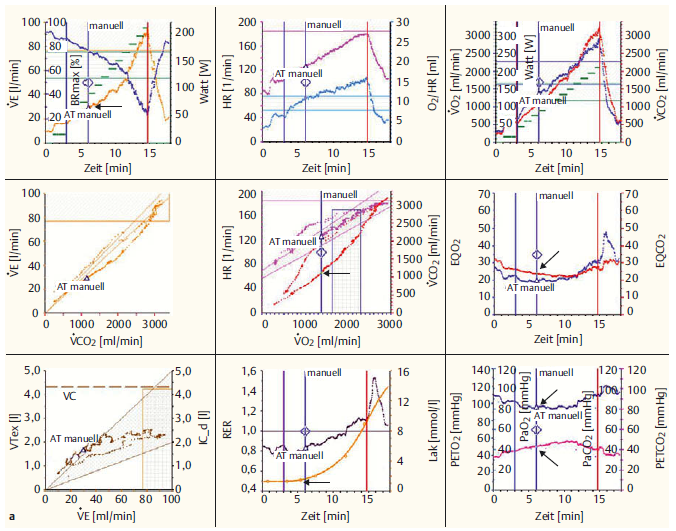
\includegraphics[width=7cm]{Bilder/9fieldcomplex.png}
\caption{Beispiel einer 9-Felder-Grafik nach einer Spiroergometrie mit einer jungen sportlichen Frau}
\end{figure}
\end{frame}

\begin{frame}{Spiroergometrie: 9-Felder-Grafik}
\begin{itemize}
\item grafisches Instrument der Spiroergometrie zum Vergleich vieler unterschiedlicher Messwerte
\item Nummerierung von oben links nach unten rechts von eins bis neun
\item kann je nach diagnostischem Schwerpunkt sehr komplex werden
\item in der Sportmedizin sind nur bestimmte Felder relevant: Fokus auf Feld 4, 5, 6 und 9 (Scharhag-Rosenberger, 2013)
\item Grafik muss auf Darstellung der ventilatorischen Schwellen reduziert werden
\item mehrere existente Methoden zur Schwellenbestimmung
\end{itemize}
\end{frame}

\begin{frame}{Spiroergometrie: Methoden zur Schwellenbestimmung}
\begin{itemize}
\item wissenschaftlich renommierteste Methoden wurden von AG Spiroergometrie zusammengefasst (Westhoff et al., 2012)
\item zwei Methoden für jede Schwelle werden in dieser Arbeit untersucht
\end{itemize}
\begin{columns}
\begin{column}{5cm}
\begin{block}{VT1}
\begin{enumerate}
\item V-Slope: erster überproportionaler Anstieg der $\dot{V}CO_2$ gegenüber der $\dot{V}O_2$
\item alleiniger Anstieg des Sauerstoff-Äquivalents $EQO_2$
\end{enumerate}
\end{block}
\end{column}
\begin{column}{5cm}
\begin{block}{VT2}
\begin{enumerate}
\item überproportionaler Anstieg der $\dot{V}E$ gegenüber der $\dot{V}CO_2$
\item Anstieg des Kohlenstoffdioxid-Äquivalents $EQCO_2$
\end{enumerate}
\end{block}
\end{column}
\end{columns}
\end{frame}

\begin{frame}{Spiroergometrie: Bestimmung der VT1}
\begin{columns}
\begin{column}{5cm}
\begin{figure}[H]
\begin{center}
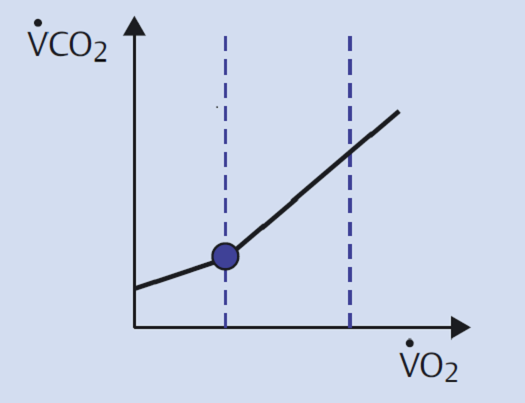
\includegraphics[width=40mm]{Bilder/vslope.png}
\caption{Schematische Darstellung der V-Slope-Methode}
\end{center}
\end{figure}
\end{column}
\begin{column}{5cm}
\begin{figure}[H]
\begin{center}
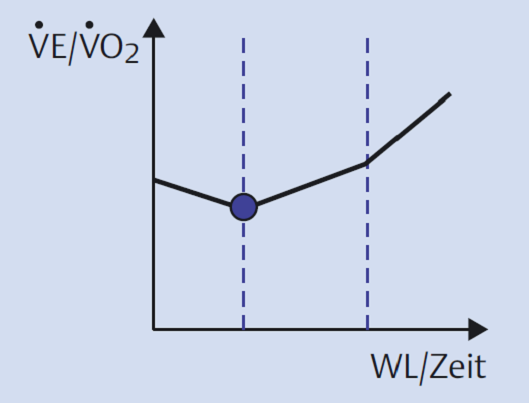
\includegraphics[width=40mm]{Bilder/eqo2.png}
\caption{Schematische Darstellung des EQO\textsubscript{2}}
\end{center}
\end{figure}
\end{column}
\end{columns}
\end{frame}

\end{document}